
\hypertarget{learn-by-building}{%
	\section{Learn by building}\label{learn-by-building}}

The mechanics and biology of epithelial tissues are complex, with mechano-chemical signaling and multiscale behavior all intertwined. The lens of active material has been instrumental in illuminating the role of molecular elements in undergoing shape changes during morphogenesis. Mechanistic understanding has been enhanced with new mathematical tools and advanced microscopy, enabling measurement of the forces involved in tissues.

The traditional and successful method for studying mechanics has been to deconstruct the system one component or parameter at a time. By manipulating genes or disrupting cellular processes, we can observe how mechanics change. This perturbative method allows for the alteration of biological systems at various levels, from molecular to tissue, (see fig \ref{fig_4_1}) .

However, studying systems like organoids or embryos can only provide limited physical insights into the topological transitions of these structures, as experimental systems have limited physical control and ability to measure forces. An alternative approach is to learn by actively performing morphogenesis or reconstructing biological structures from their basic components.

\begin{figure}
	\centering
	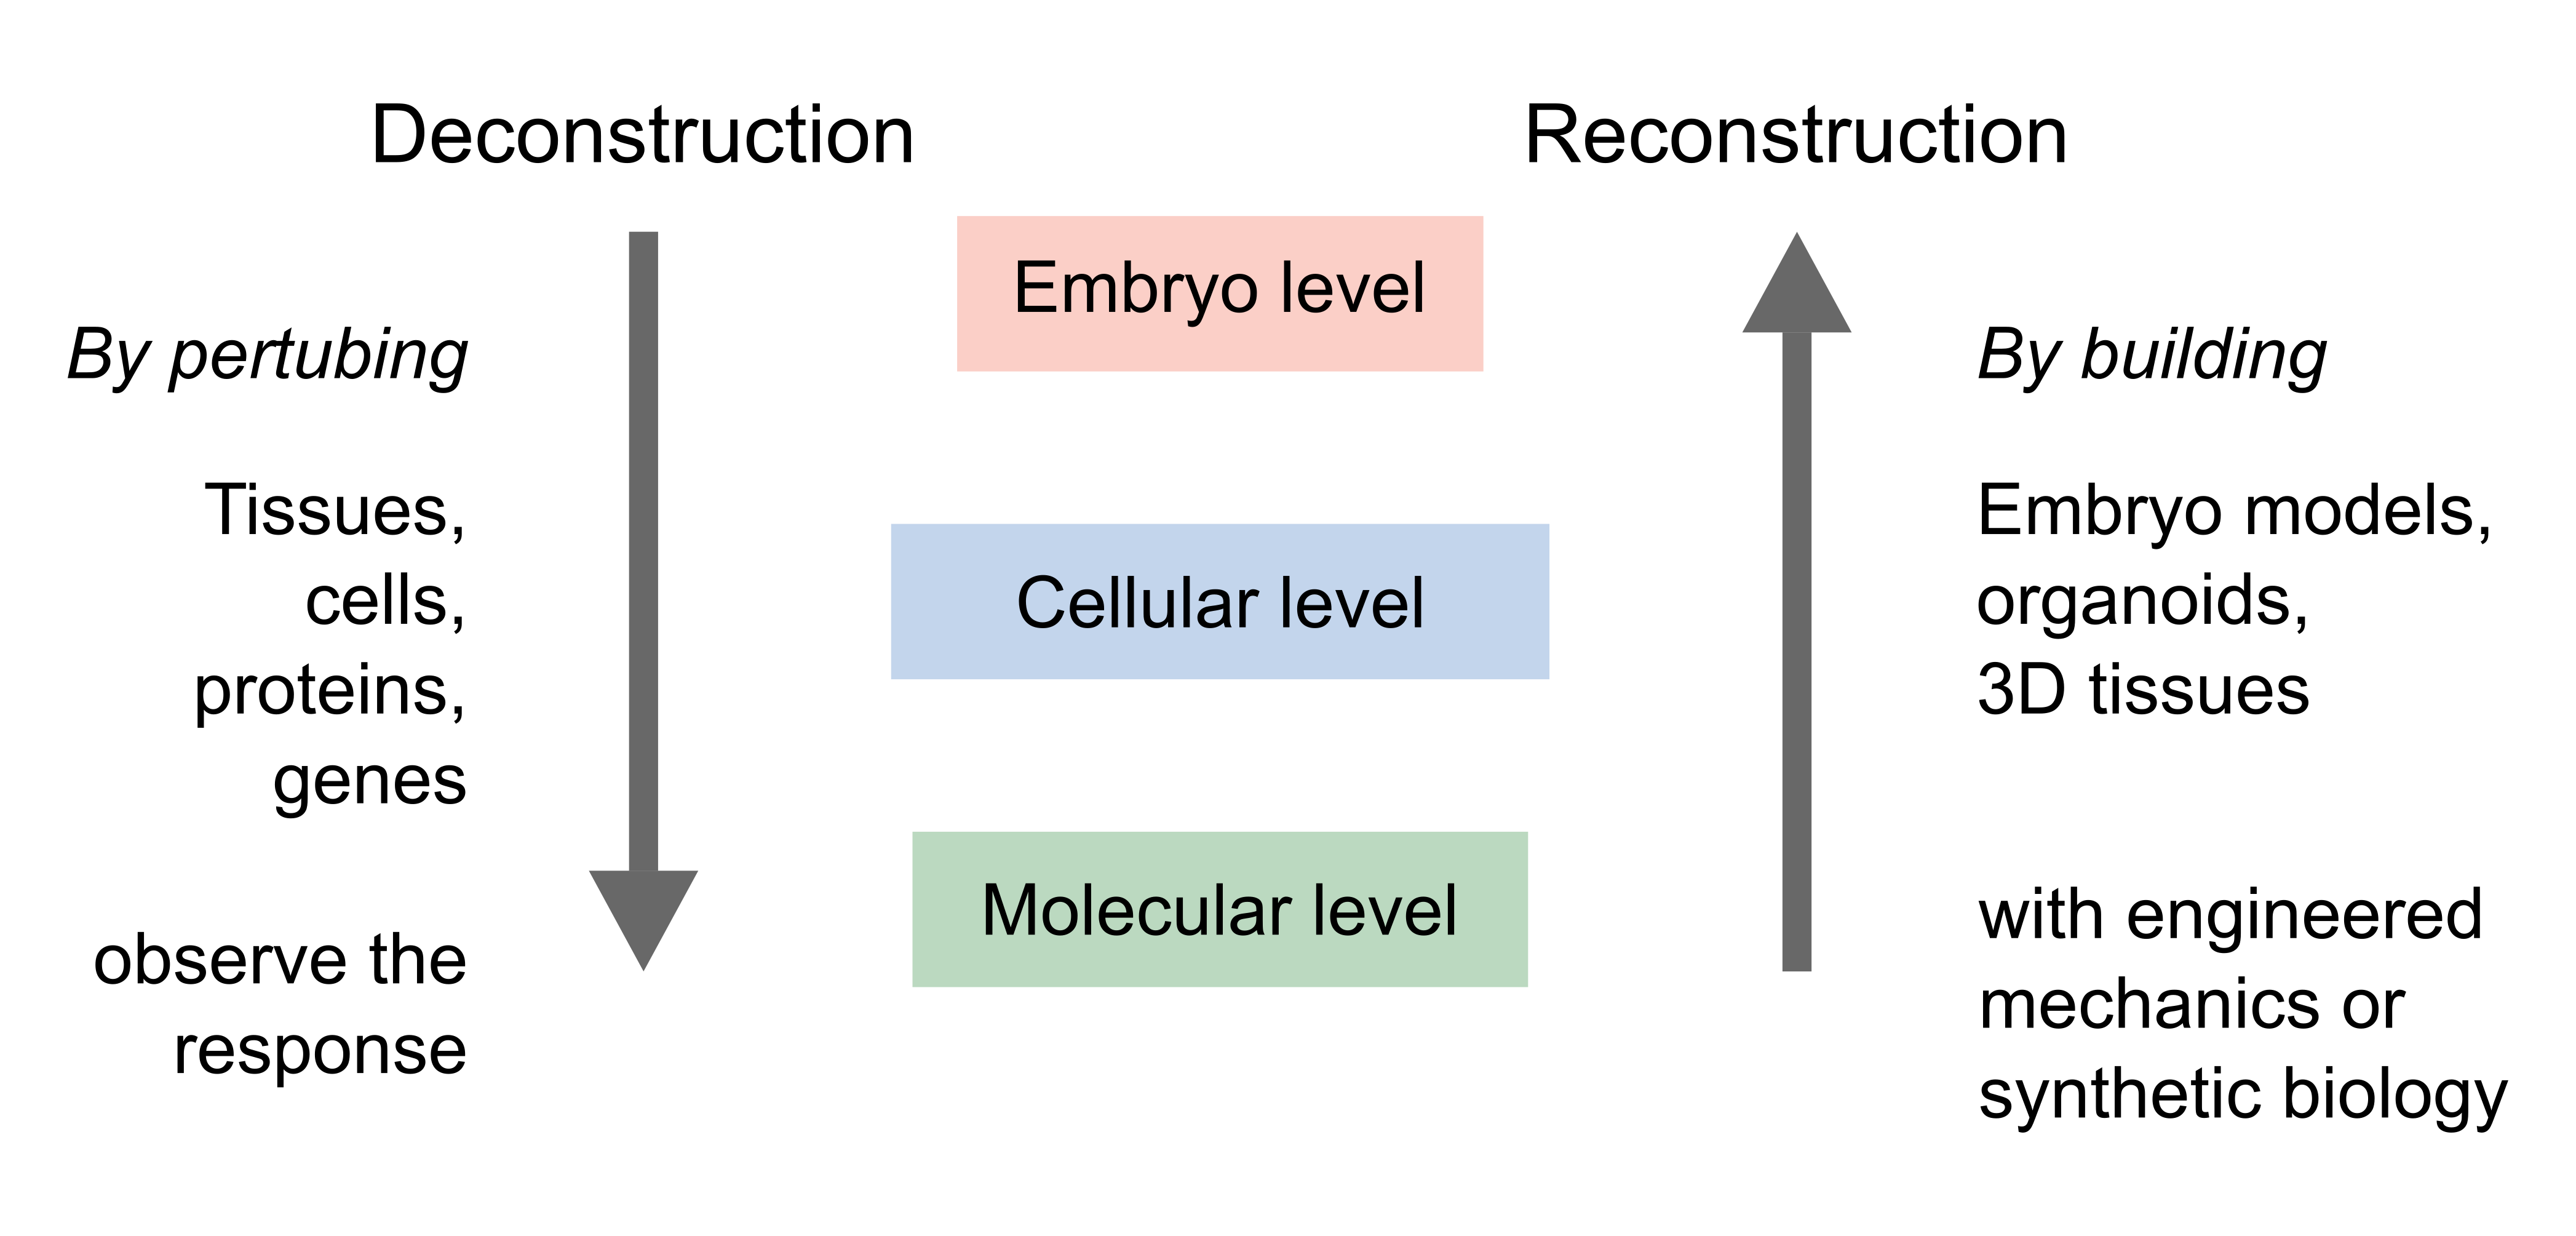
\includegraphics[width=0.65\textwidth]{chap4building.png}
	\caption{\label{fig_4_1} \textbf{A conceptual representation of two approaches to understanding mechanics: reconstruction (bottom-up) and deconstruction (top-down).} In reality, they are not separate from each other. These methods inform each other, with past top-down research guiding new reconstruction, and new engineered cells or tissues furthering our understanding of the field in innovative directions.
}
\end{figure}

For years, researchers have broken down biological systems into approachable parts - tissues, cells, proteins - in order to understand the behavior of each component. However, combining existing knowledge of these parts to recreate novel experimental systems could reveal the basic building blocks and effects of scale. This approach would complement top-down approaches in developmental biology. Synthetic biology, a perfect example of reconstruction, seeks to recreate life at various scales, from synthetic proteins to entire cells, in order to gain a deeper understanding of the indispensable components of life.

As active agents exist at every scale, emergent properties can appear at higher scales. Thus, it is essential to focus on higher scales or work with collectives of cells. This reminds me of the example of cars and traffic: Imagine you know the behavior of all individual car components, but this information is not sufficient to understand the behavior of traffic flow. This requires a higher level of analysis. 
\footnote{Matthew Good's commentary provides an insightful perspective on the complexity involved in building cells from interacting molecules. Meanwhile, Xavier Trepat argues that a bottom-up approach does not fully explain the emergent behavior of higher-level structures and emphasizes the need for constructing tissues at the mesoscale. Trepat uses the analogy of traffic jams to illustrate the importance of considering the collective behavior of cells in tissue engineering \cite{good2018}.} 
Similarly, biological structures exhibit numerous collective behaviors, such as jamming, nematic order, instabilities, or self-organization \cite{trepat2018}. 

Recreating structures from scratch also provides an opportunity to understand the role of physics at different scales. In the spirit of D'Arcy Thompson, we can explore the fundamental properties of matter in biological structures.
\footnote{. Thompson writes,’...to seek not for ends but for antecedents is the way of the physicists, who finds causes in what he has learned to recognize as fundamental properties, or inseparable concomitants, or unchanging laws, of matter and of energy.” \cite{thompson1979}}
For instance, we can study the role of surface tension in guiding the shape of cellular aggregates or lumens. In this work, we focus on the mesoscale structures of epithelia \((\sim 10-10^4 \mu m)\).  

We present our efforts to engineer an epithelial structure with a controlled microenvironment that is sensitive to self-organization and mechanical instabilities. The following sections will describe the ways of creating these structures from minimal ingredients.

\hypertarget{how-to-build-tissue-structures}{%
	\section{How to build tissue 		structures?}\label{how-to-build-tissue-structures}}

Before embarking on the construction of a tissue structure, it is important to consider the desired form and function. Despite the diversity in the shapes and functions of tissues, certain elementary shapes can be seen in many cases, resulting from the interplay between physical forces and biochemical signaling. Examples of such shapes include spherical blastocysts, ellipsoidal embryos, or cylindrical vessels.

After considering the desired form and function of the structure, established cell lines are selected and synthetic structures are constructed using various techniques, such as geometry control and localized folding, as discussed in the \ref{mechanobiology} section. The resulting structures can be further studied to understand the interplay between physical forces and biochemical signaling, as well as their potential applications in various biological systems.

\hypertarget{controlling-geometry-and-physical-forces}{%
	\subsection{Controlling geometry and physical 		forces}\label{controlling-geometry-and-physical-forces}}

From an engineering perspective, scaffolding is a commonly used approach for constructing synthetic epithelial structures. Scaffolds can be generated through 3D printing or microfabrication techniques, and cells can then be seeded onto the scaffold to attain the desired shape \cite{torras2018}. This method allows for the creation of a well-controlled microenvironment for the cells in terms of geometry, stiffness, adhesion proteins, and cell culture media (see fig \ref{fig_4_2} A) . Structures generated through this approach can be utilized to investigate tissue behavior in response to forces and curvature.

For instance, cells can be used to form a micro-vessel using a hydrogel with a cylindrical hole \cite{dessalles2021}. The hydrogel and cells were housed in a microfluidic device that controlled pressure and flow in the vessel, and the authors were able to examine the role of hydrogel poroelastic properties in regulating the dynamics of the vessel. Another exciting study demonstrated the potential of epithelial tissues to form shape-programmable materials by using a collagen scaffold \cite{mailand2022}.

Scaffolds can also be designed to dynamically change their shape (see fig \ref{fig_4_2} B). For example, a cell monolayer on a flexible membrane can alter its curvature \cite{blonski2021}, and a combination of stretching and unstretching a cell-laden hydrogel can produce distinctive folds and patterns \cite{chan2018}. In some cutting-edge studies, researchers have utilized 4D bioprinting, where 3D printed objects undergo transformation over time \cite{arif2022}. For instance, a flat hydrogel sheet containing endothelial cells and photo-crosslinking can be transformed into a tube \cite{zhang2020}.


\begin{figure}
\centering
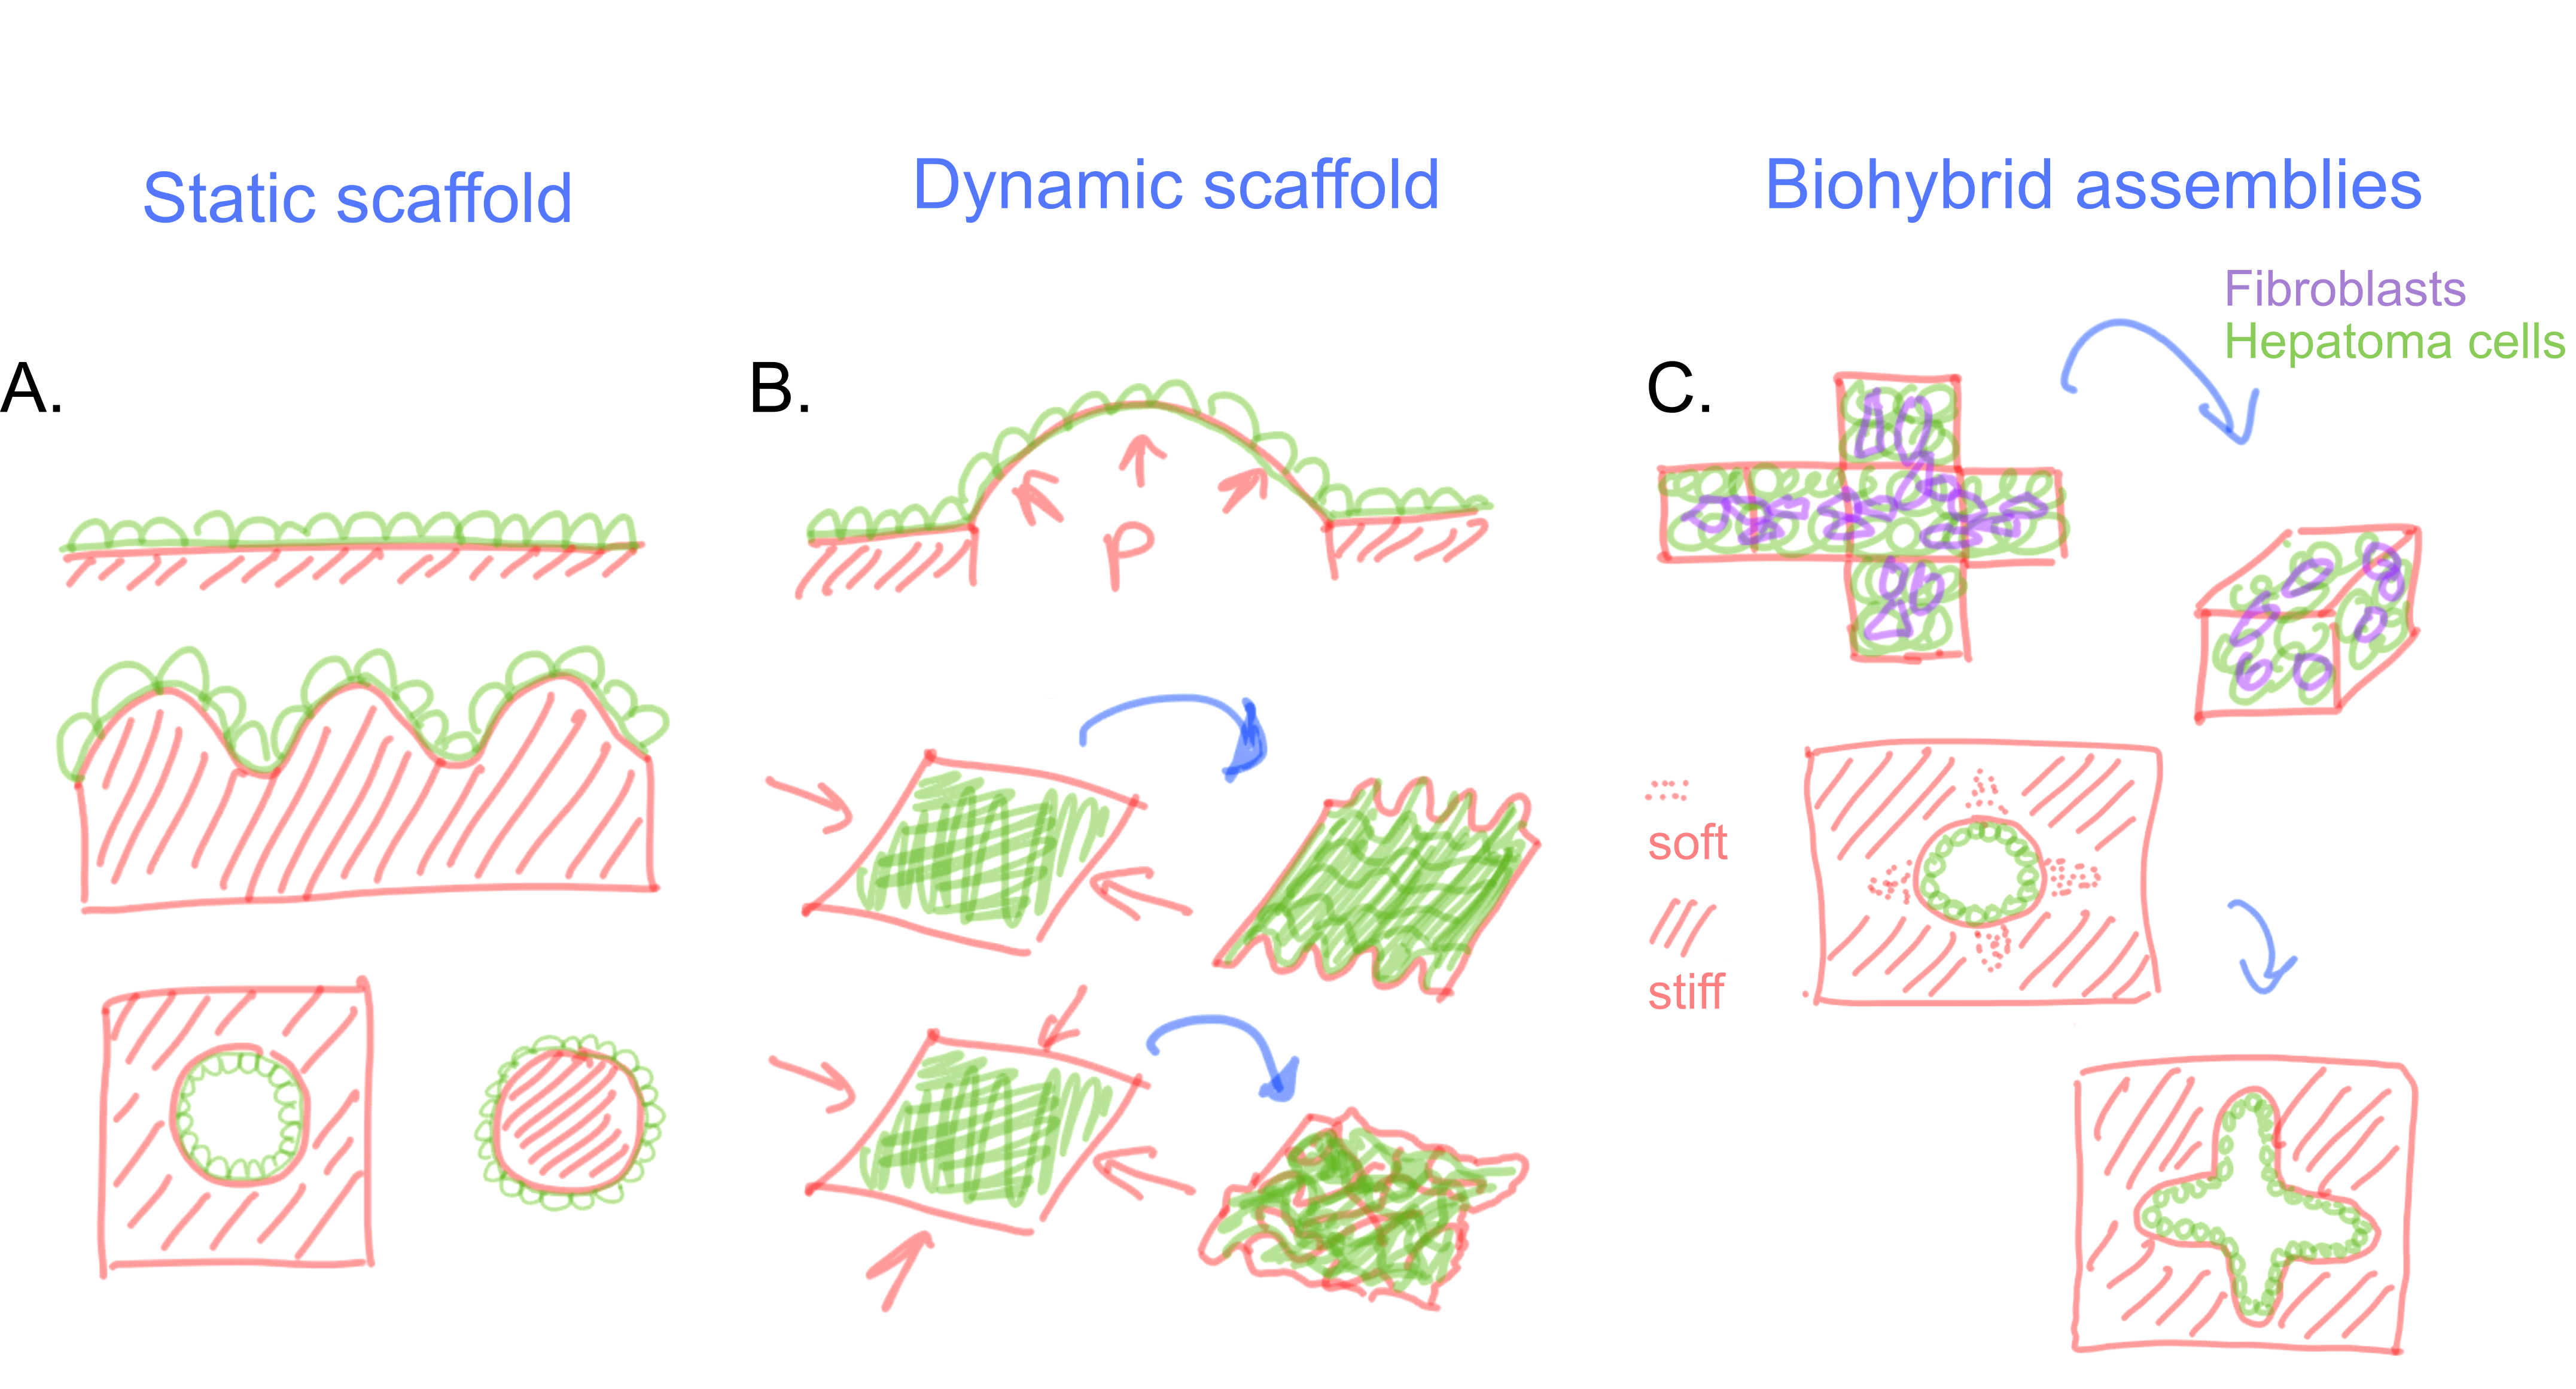
\includegraphics[width=\textwidth]{chap4scaffold.png}
\caption{\label{fig_4_2}\textbf{Controlling geometry and physical forces: } The concept of scaffolding can be divided into two categories: static and dynamic scaffolds. (A) Static scaffolds are microfabricated structures that cells can adapt to and respond to geometrical cues, leading to the formation of a specific tissue organization \cite{brassard2021}. (B) In contrast, dynamic scaffolds consist of cell-laden matrices that are deformable, and their curvature can change dynamically due to external pressure or mechanical forces \cite{blonski2021, chan2018}. (C) Biohybrid assemblies can incorporate active contraction or pushing to create hybrid structures, such as origami folding triggered by fibroblast contraction \cite{he2018}, or cells carving out an intestinal crypt-like geometry from a softer matrix \cite{gjorevski2016}.}
\end{figure}

Additionally, the contractility of fibroblasts and hepatoma cells has been utilized to fold 2D structures into 3D shapes \cite{he2018} (see fig \ref{fig_4_2} C) . Microplates with an origami folding pattern are created, and the cells apply forces to generate a 3D structure. In other scenarios, cells are allowed to self-organize through the imposition of geometric constraints, which enhances the efficiency of organoid-like systems \cite{gjorevski2016}. In the case of intestinal organoids, controlling the stiffness of the matrix in specific regions leads to growth and differentiation at softer areas, producing a highly reproducible structure \cite{gjorevski2022}.

\hypertarget{manipulating-biochemical-signaling}{%
	\subsection{Manipulating biochemical signaling}\label{manipulating-biochemical-signaling}}

Another approach to constructing biological structures involves controlling biochemical signaling to induce shape transformation. This approach utilizes natural processes in embryo morphogenesis, such as apical constriction in ventral furrow formation or cell jamming in the normal elongation of the zebrafish. Optogenetic tools, such as controlling Rho signaling, can be used to induce localized apical constriction with spatiotemporal control \cite{izquierdo2018}. This technique can also be applied to other proteins, such as Shroom3, to induce synthetic morphogenesis in neural organoids \cite{martinez-ara2022} (see fig \ref{fig_4_3} C).

Epithelial-mesenchymal interaction is another crucial aspect of the tissue folding process. Hughes et al. demonstrated that cell clusters can remodel the matrix to create oriented stresses that lead to budding in tissues \cite{hughes2018}. By controlling the location and density of these cell clusters, it is possible to manipulate the curvature of the epithelia. Mesenchymal condensation serves as a folding template for the final tissue structure \cite{palmquist2022, shyer2017} (see fig \ref{fig_4_3} B).

The microenvironment plays a critical role in providing vital signals to tissues and can be manipulated to activate specific cellular functions. Microfluidic techniques can deliver appropriate morphogen gradients to the tissue with precise timing \cite{hofer2021}. \textit{In vivo}, multiple morphogens often act simultaneously. For instance, during neural tube development, there is an opposing gradient of sonic hedgehog (SHH) and bone morphogenic protein (BMP). With microfluidic devices, stable gradients can be generated, even in opposite directions \cite{demers2016}, thus mimicking symmetry-breaking events and directional neural tube patterning (see fig \ref{fig_4_3} D).

Moreover, genetic engineering of specific cells can be utilized to control signaling. Human pluripotent stem cells (hPSCs) can be programmed to express SHH \cite{cederquist2019} (see fig \ref{fig_4_3} E). Mixing these cells with others could result in a polarized organoid and a patterned cerebral organoid.

\begin{figure}
	\centering
	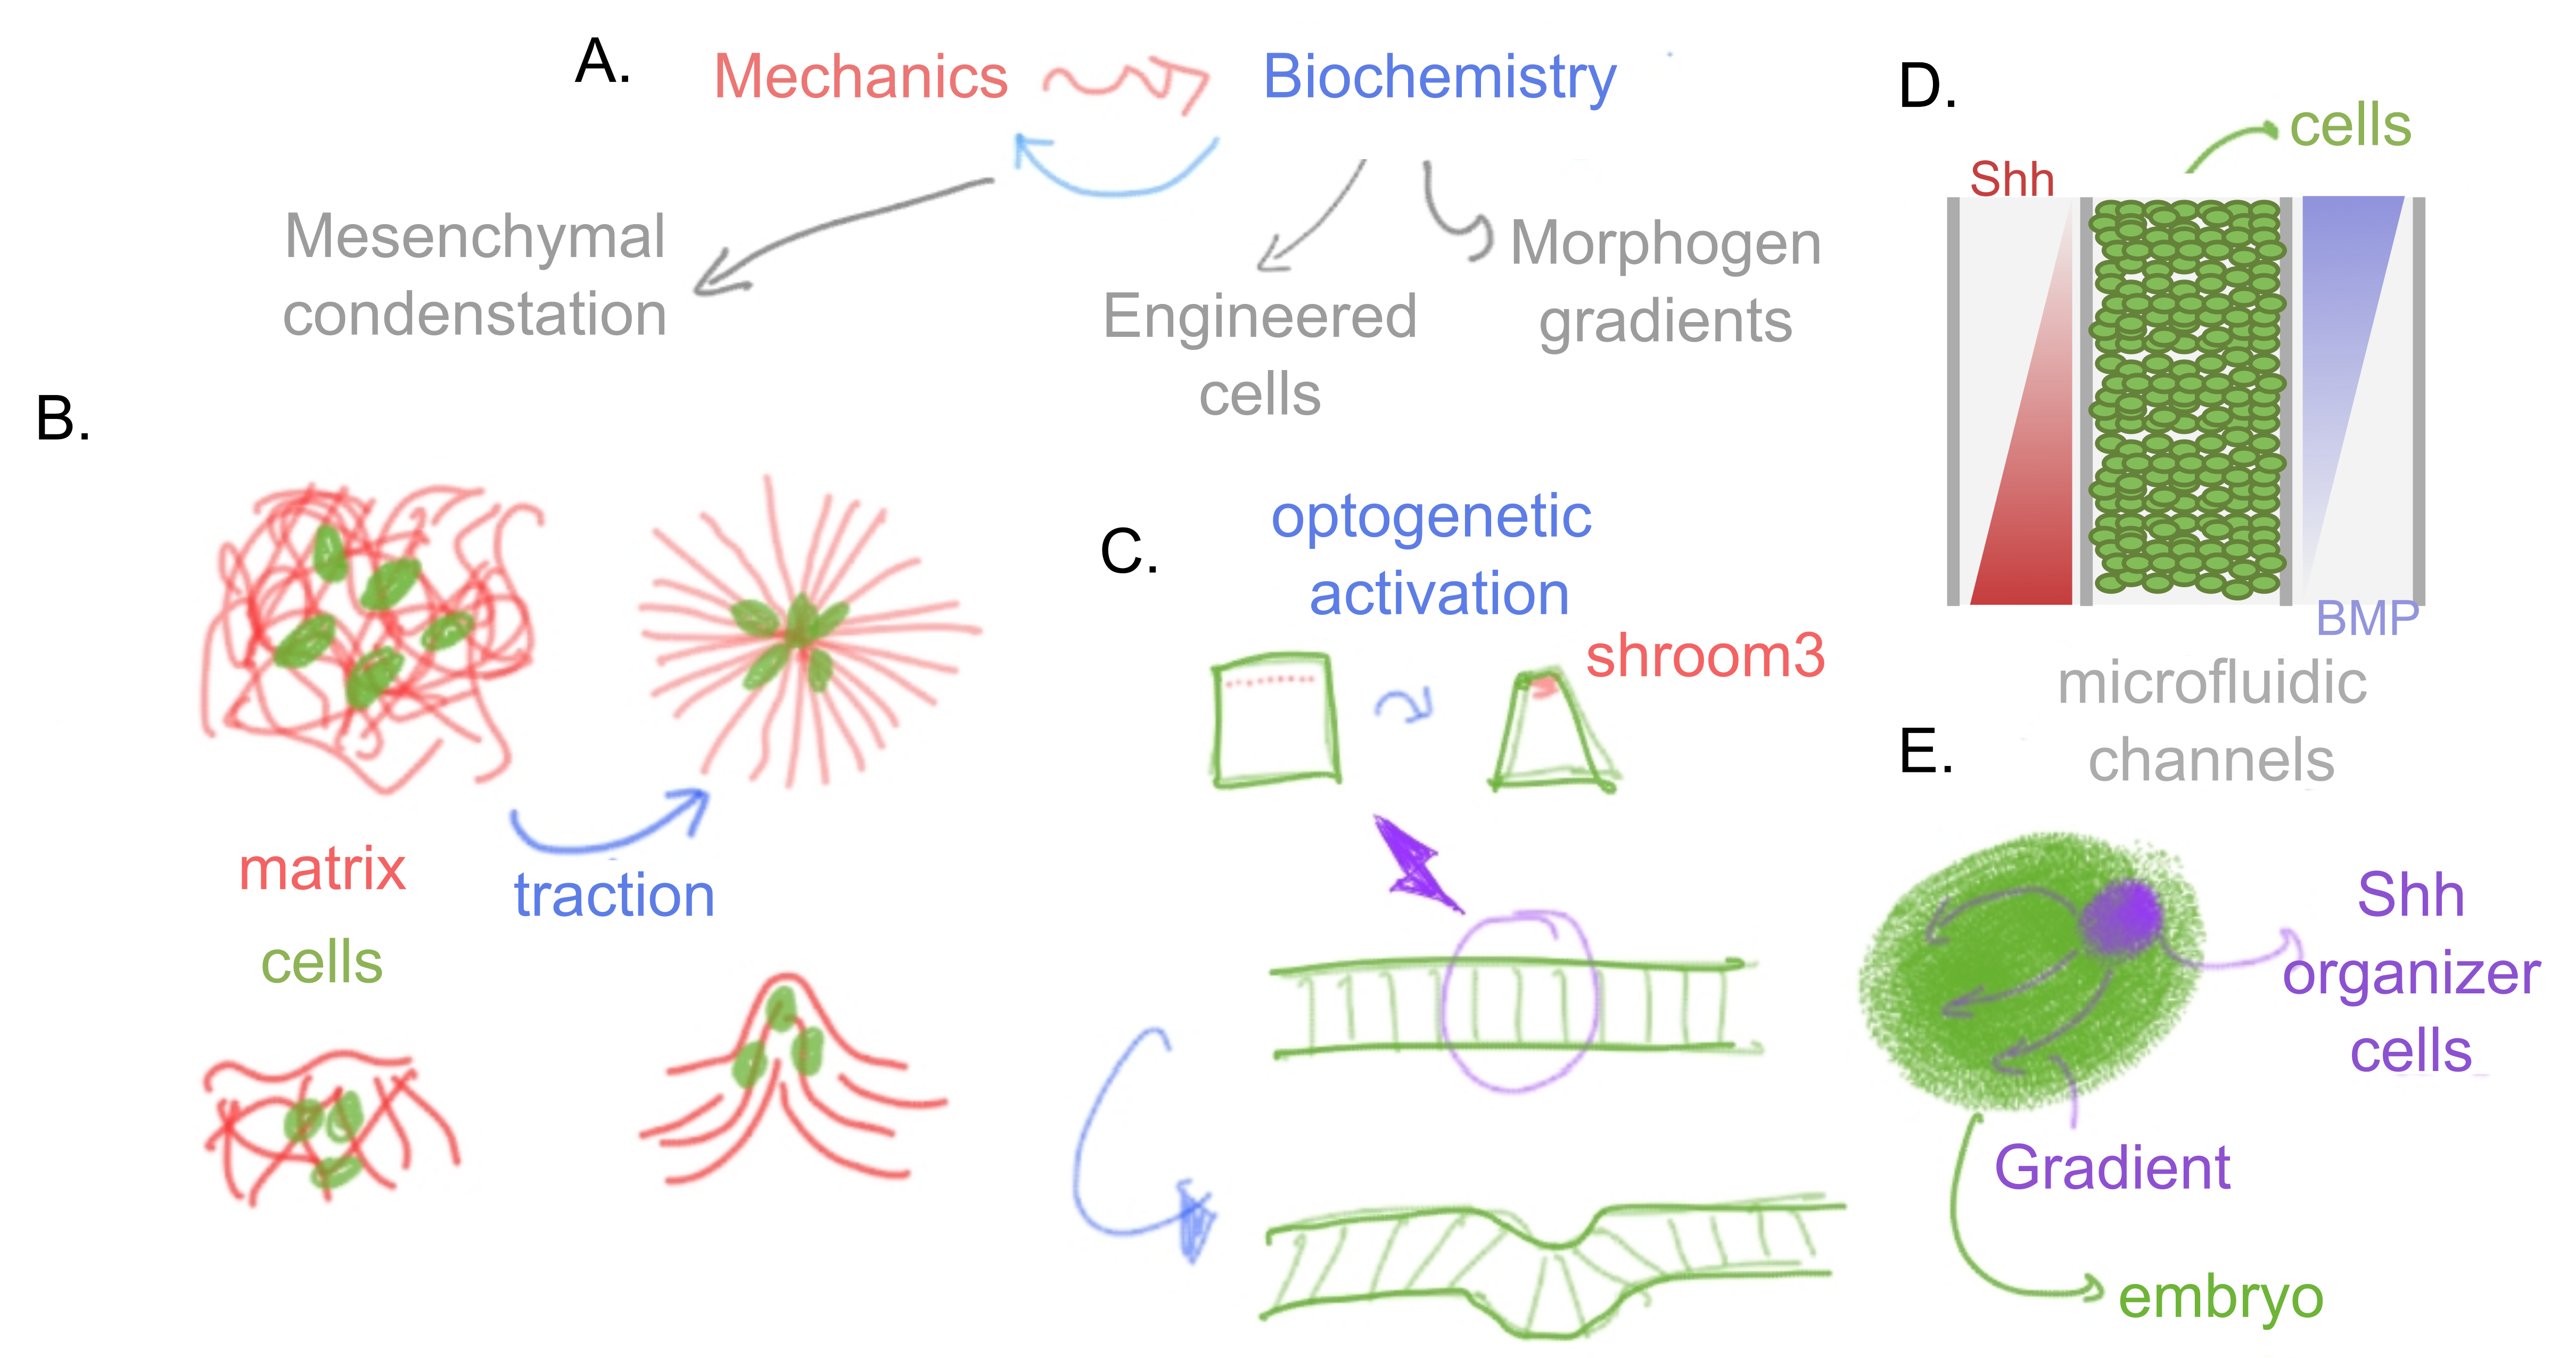
\includegraphics[width=\textwidth]{chap4biochem.png}
	\caption{\label{fig_4_3} \textbf{Manipulating biochemical signaling:} Biochemical signaling and mechanics are interdependent in morphogenetic processes (A). The transport of signaling molecules can affect the cytoskeleton and mechanical properties of cells, while mechanical forces can also influence biochemical signaling. Microfluidics (D) is one method used to control biochemical signaling by providing opposing morphogen gradients through multiple channels \cite{demers2016}. Alternatively, cells can be genetically engineered to undergo apical constriction (C) or produce morphogen gradients (E) locally to form curved geometries \cite{martinez-ara2022, cederquist2019}. Mesenchyme condensation (B) is another approach used to program curvature in developing tissues \cite{hughes2018, palmquist2022}.}
\end{figure}

\hypertarget{exploiting-mechanical-instabilities}{%
	\subsection{Exploiting mechanical
		instabilities}\label{exploiting-mechanical-instabilities}}

\begin{figure}
	\centering
	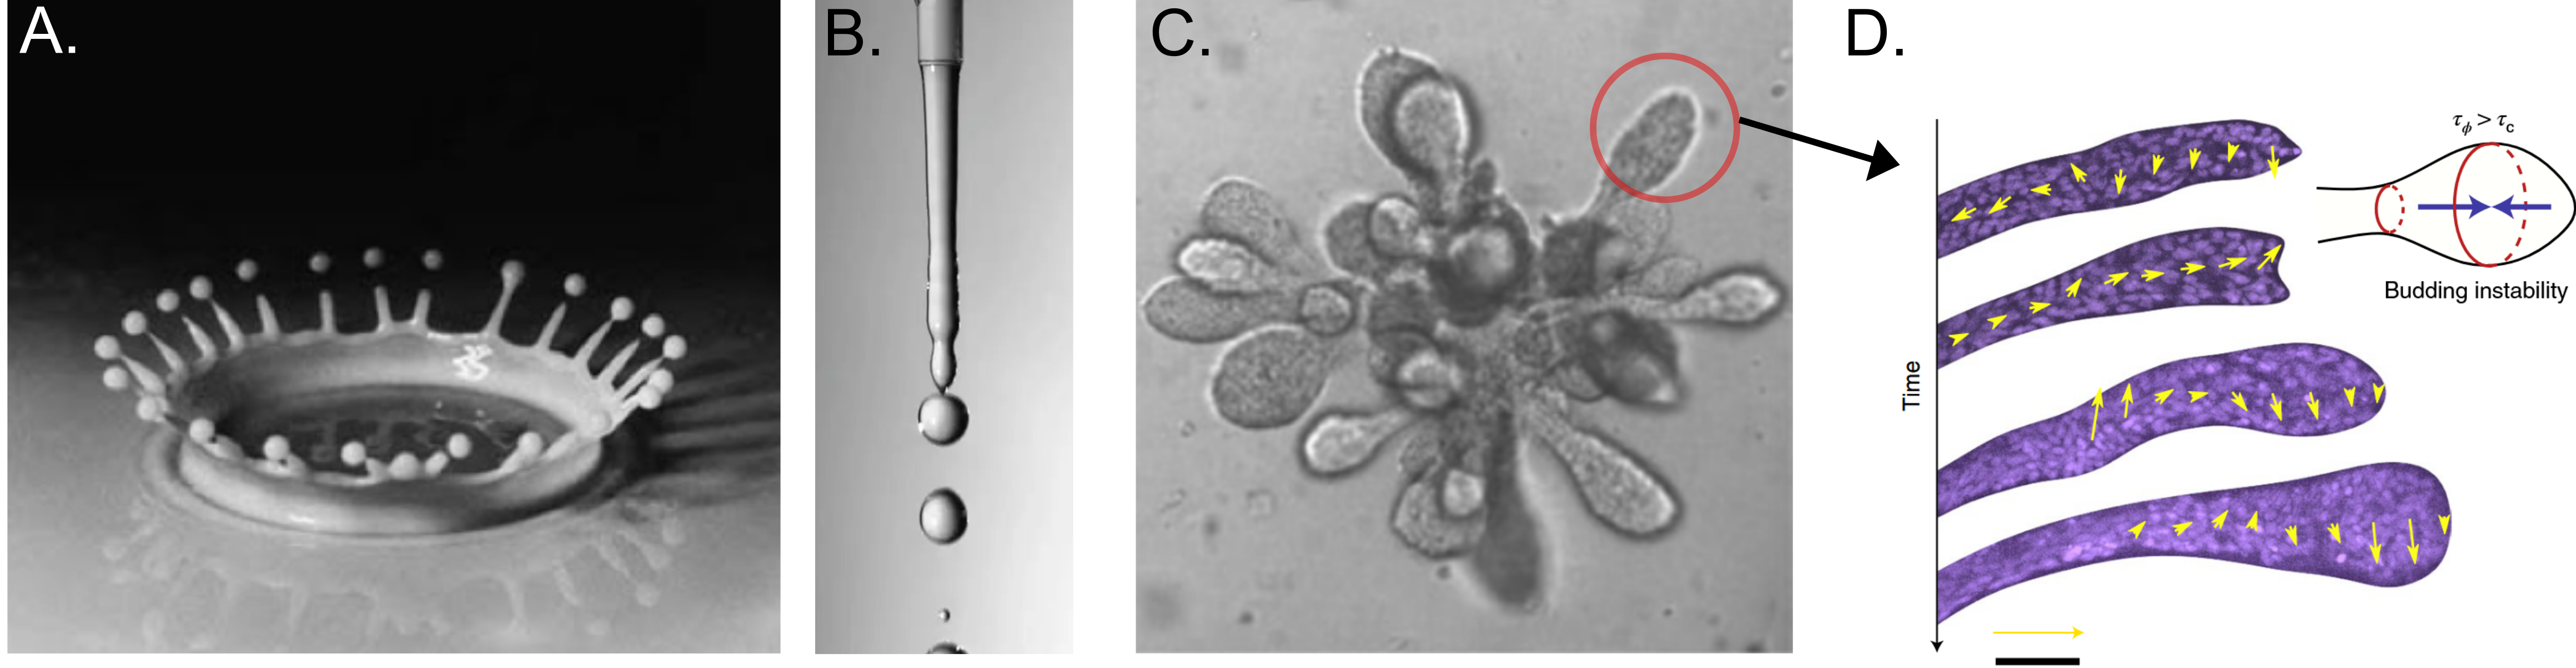
\includegraphics[width=\textwidth]{chap4rayleigh.png}
	\caption{\label{fig_4_4} \textbf{D'Arcy Thompson compares biological budding to splashes} (A) of fluids and Rayleigh-Plateau instability \cite{thompson1979} (B), where liquid splits up into smaller droplets. This mechanism could also be seen in organogenesis of mammary tissue (C, D) \cite{fernandez2021}.}
\end{figure}

Morphogenesis, the process of shaping and formation of biological structures, often involves spontaneous pattern formation or symmetry-breaking events \cite{ishihara2018}. These processes are often dictated by mechanical instabilities, which can lead to large deformations in soft matter systems. In material science, these instabilities are typically seen as problematic as they cause rapid breakage. However, in soft matter, large deformations can lead to interesting topological transformations, providing an opportunity for engineers to exploit these instabilities in the development of new actuators or soft robots (reviewed in \cite{pal2021}).
\footnote{"Mechanical instabilities have provided a unique approach to imbue “material intelligence” into soft machines without requiring the addition of rigid components. For example, binary actuators relying on mechanical instabilities can recreate logic modules and reproduce valving functionality using entirely soft elements.}

The significance of mechanical instabilities was foreseen by D'Arcy Thompson in his comparison of fluid splashes to hydroids (see fig \ref{fig_4_4} A). He wrote that the shapes of a potter's cup, glass blower's bulb, and biological structures are simply glorified splashes formed slowly under conditions of restraint that enhance or reveal their mathematical symmetry \cite{thompson1979}.
\footnote{ I cannot recommend enough the chapter “the forms of cell”. He states “Many forms are capable of realization under surface-tension, … The subject is a very general one; it is, in its essence, more mathematical than physical; it is part of the mathematics of surfaces, and only comes into relation with surface-tension because this physical phenomenon illustrates and exemplifies, in a concrete way, the simple and symmetrical conditions with which the mathematical theory is capable of dealing.”}
This conjecture has been confirmed through numerous quantitative studies on various systems, including ripples in leaves and wrinkles in the brain \cite{liang2009, karzbrun2018}.

There are various instabilities associated with solids and fluids. For example, the Rayleigh-Plateau instability explains why a fluid stream breaks into smaller packets, driven by the fluid's tendency to minimize its surface area due to surface tension. The same instability can arise when fluid is surrounded by an elastic medium, instead of air, provided the surface tensions can overcome the elastic stresses, leading to budding as observed in alveologenesis in human mammary tissue \cite{fernandez2021} (see fig \ref{fig_4_4} C-D). However, as tissues are active viscoelastic materials surrounded by viscoelastic medium, the timescales of these instabilities change, slowing down to hours instead of milliseconds in water droplets.

There are several types of mechanical instabilities associated with solids and fluids, including Rayleigh-Plateau instability, Kelvin-Helmholtz instability, Rayleigh-Taylor instability, viscous coiling and folding, and large-scale wrinkling and buckling \cite{gallaire2017, kourouklis2018}. In this study, we aim to harness these instabilities to recreate epithelial structures.

Applying compressive stresses is one of the easiest ways to induce mechanical instabilities in solids. These stresses can occur in biological systems as a result of differential growth, swelling, or morphogen gradients and can lead to various forms of instabilities, including wrinkling, creasing, and buckling. Buckling occurs when a thin sheet is subjected to in-plane compressive stress, and if the stress is above a critical value, the sheet undergoes out-of-plane deformation instead of in-plane shrinkage (see fig \ref{fig_4_5} B). In contrast, wrinkling and creasing occur in similar compressive stresses, but the thin sheet is typically supported by a compliant substrate.

\begin{figure}
	\centering
	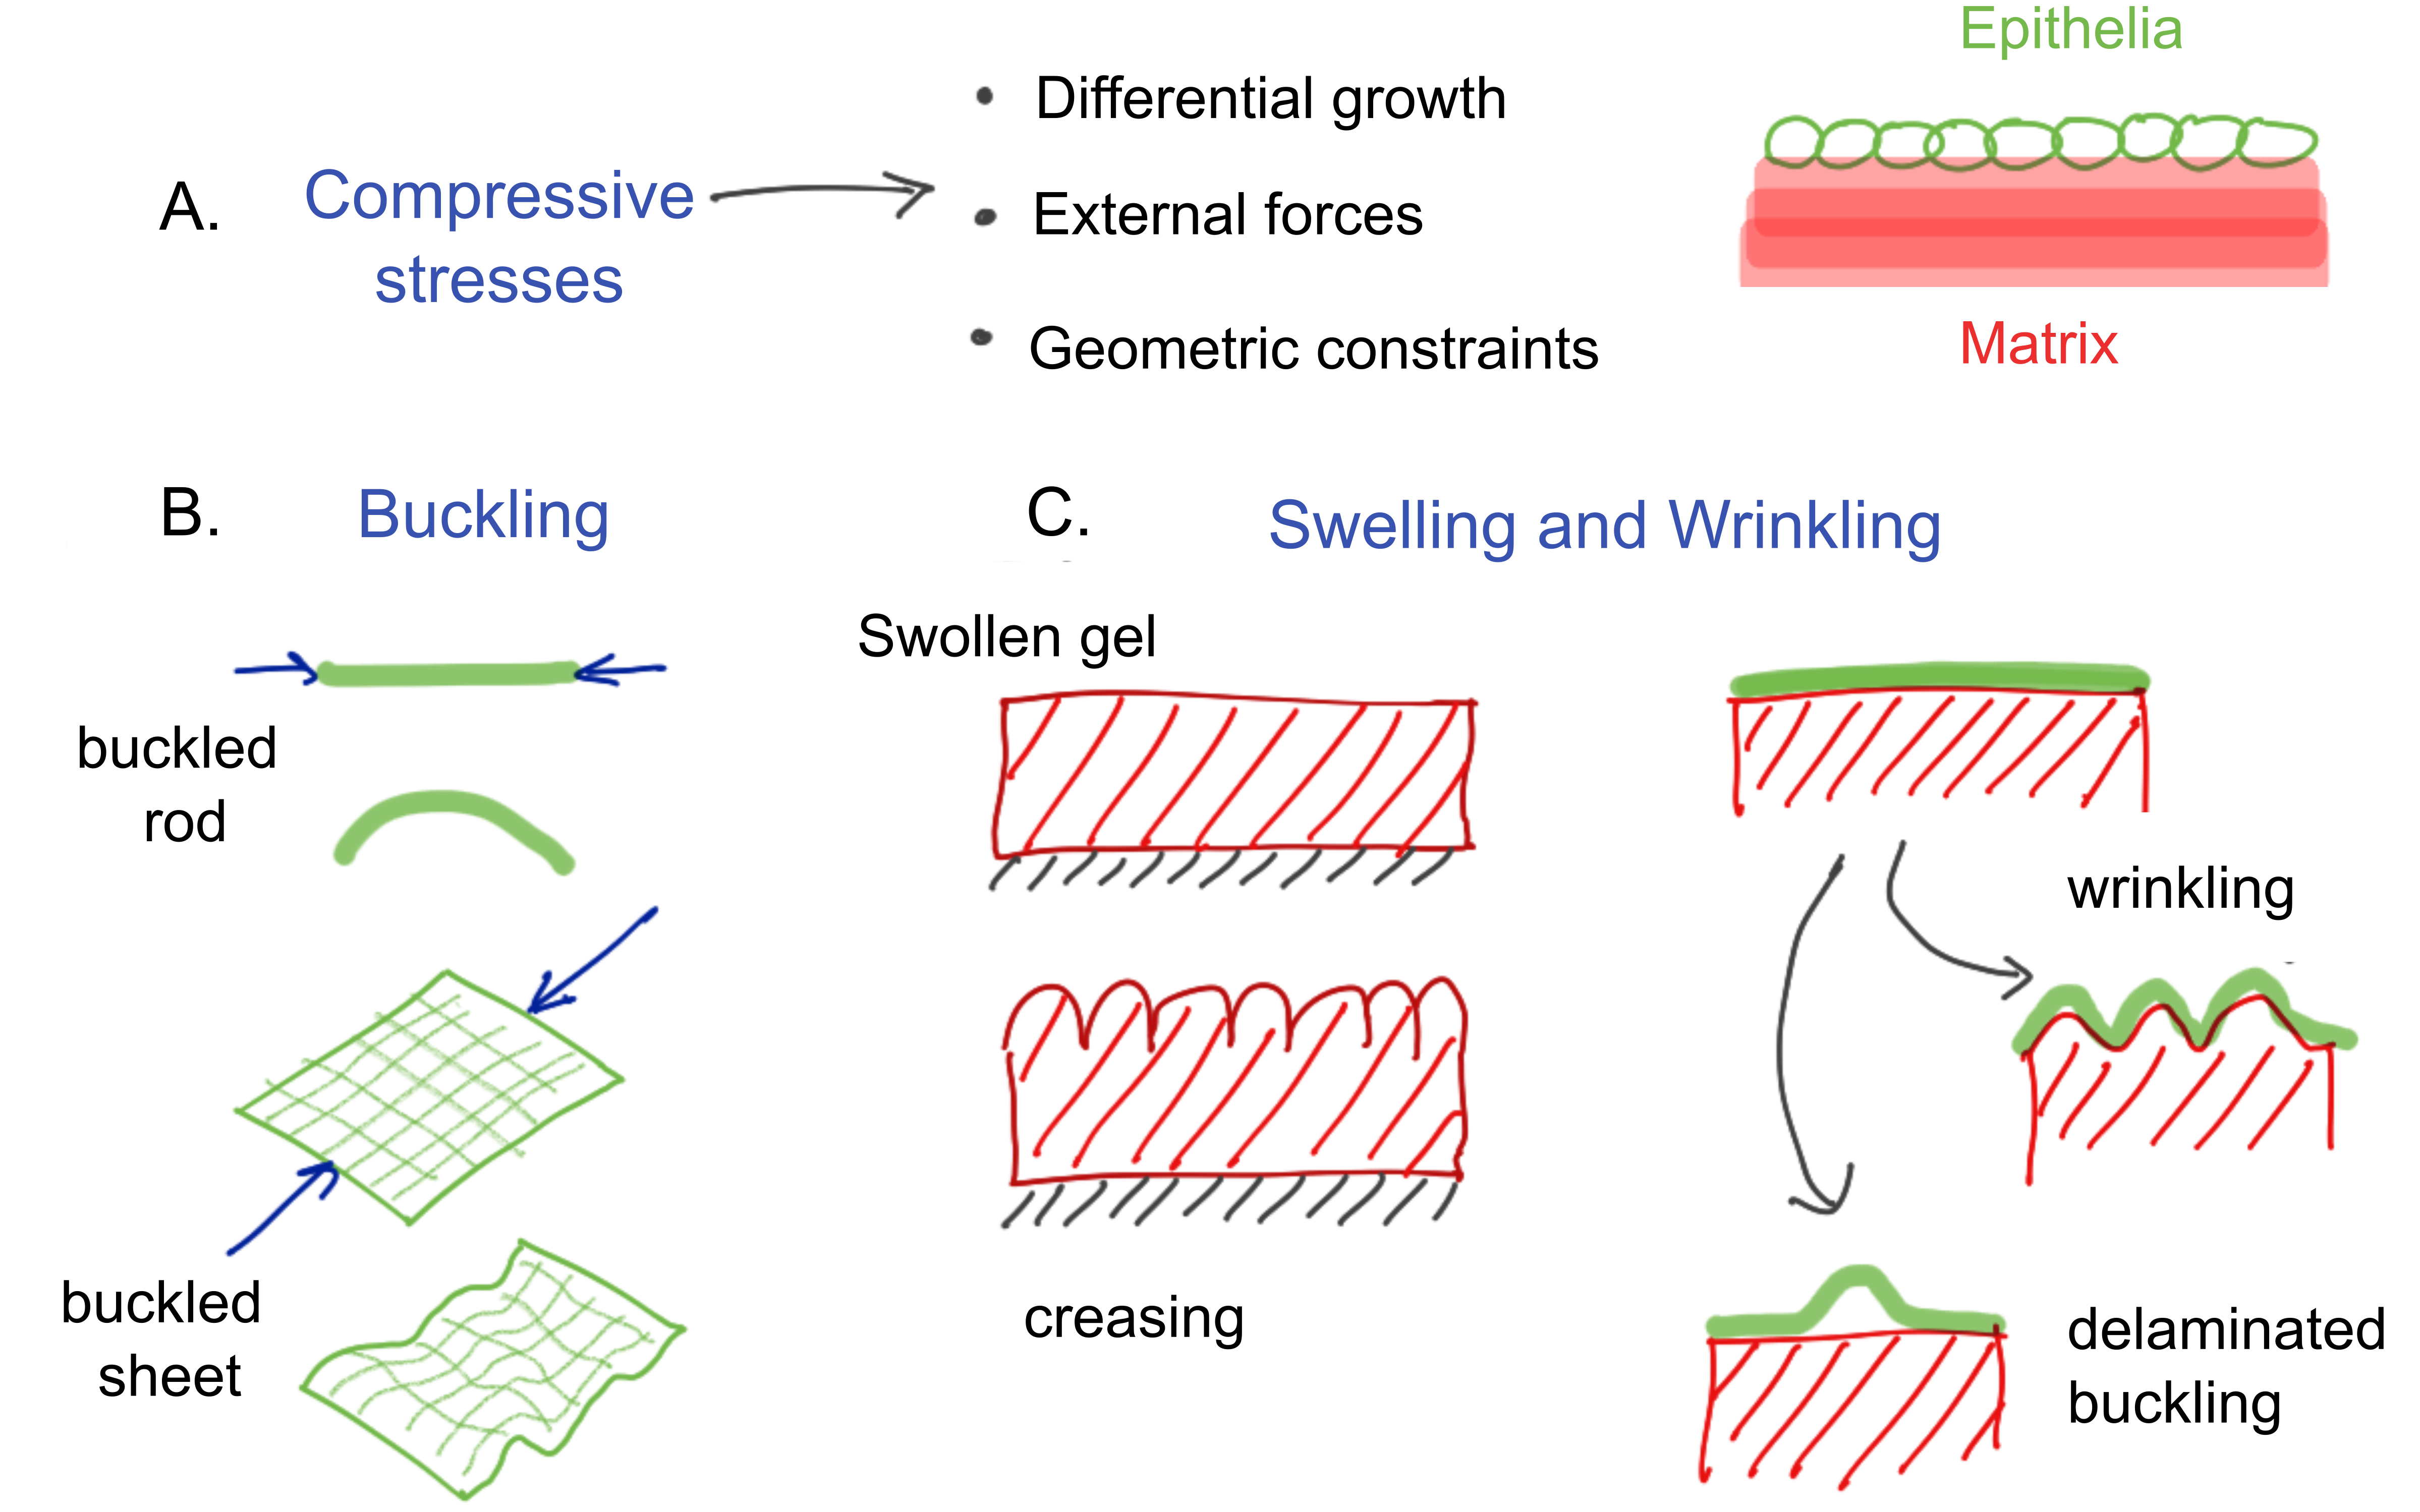
\includegraphics[width=0.8\textwidth]{chap4instabilites.png}
	\caption{\label{fig_4_5} \textbf{Compressive stresses} occur frequently in many systems (A). We can consider epithelia and matrix as thin sheet supported by a compliant substrate. Thus, the tissue folding could be understood as buckling of sheets (B) or wrinkling or creasing of thin film supported by an hydrogel (C).}
\end{figure}

The creation of biological tissues \textit{in vitro} has been a subject of great interest in the field of tissue engineering. To reproduce the characteristics of these tissues, researchers have turned to the use of hydrogels. These materials can be mechanically and chemically manipulated to simulate the behavior of biological matrices, which provide support for epithelial structures.

One of the ways in which hydrogels can be used to recreate the behavior of biological tissues is through the application of physical stress. For example, swelling of the hydrogel can cause it to undergo rapid large volumetric changes, producing crease-like patterns on the surface. If the hydrogel is constrained at the bottom, these creases can become permanent. Alternatively, if the hydrogel is supported by another flexible material, such as another hydrogel or an elastic substrate, the stresses produced during swelling will result in a wrinkling instability (see fig \ref{fig_4_5} A). These instabilities are important for understanding the formation of a variety of structures, including the gyrification of the brain cortex.

In a study by Tallinen et al., the gyrification of the brain cortex was replicated through the programming of materials to produce wrinkling \cite{tallinen2016}. The researchers created a synthetic brain with an inner core of an inert elastomer and an outer layer of a swellable elastomer. On swelling, the outer layer produced folds that closely matched the process of gyrification (see fig \ref{fig_4_6} A).

Similar mechanisms have been observed in other systems undergoing differential growth, such as the branching of lungs and formation of intestinal villi \cite{varner2015,shyer2013} (see fig \ref{fig_4_6} B,D). These findings highlight the potential of hydrogels as a tool for understanding the physical mechanisms underlying tissue development. However, it is worth noting that the mechanisms described here are the subject of ongoing research and debate in the field of developmental biology.

The ability to recreate biological tissue growth conditions \textit{in vitro} has been made possible through the use of hydrogels. Researchers have discovered that by mechanically and chemically controlling the hydrogel, they can generate desired mechanical instabilities \cite{dervaux2012}. This can be accomplished through the swelling or pre-stretching of the gel, or by manually applying compressive stresses.

One way to simulate growth is through the direct stretching or compression of the gel. Chan et al. showed that the patterns produced can be controlled by modulating the shear modulus of the hydrogel with the epithelial layer and stretch \cite{chan2018} (see fig \ref{fig_4_5} B). By pre-stretching the hydrogel before seeding cells, they were able to produce folded patterns with different wavelengths depending on the type of pre-stretching applied (uniaxial or biaxial). 

Another type of instability in bilayers is delaminated buckling, which is often observed in thin film delamination in furniture. This can be induced through compressive stresses created during growth or collective tension. Recent studies have shown that growing epithelia confined in a sphere undergo delaminated buckling after reaching a critical growth-induced stress \cite{trushko2020} (see fig \ref{fig_4_6} C), or through intercellular stresses \cite{oyama2021} or by placing a biofilm on top of the epithelial monolayer \cite{cont2020}.

\begin{figure}
	\centering
	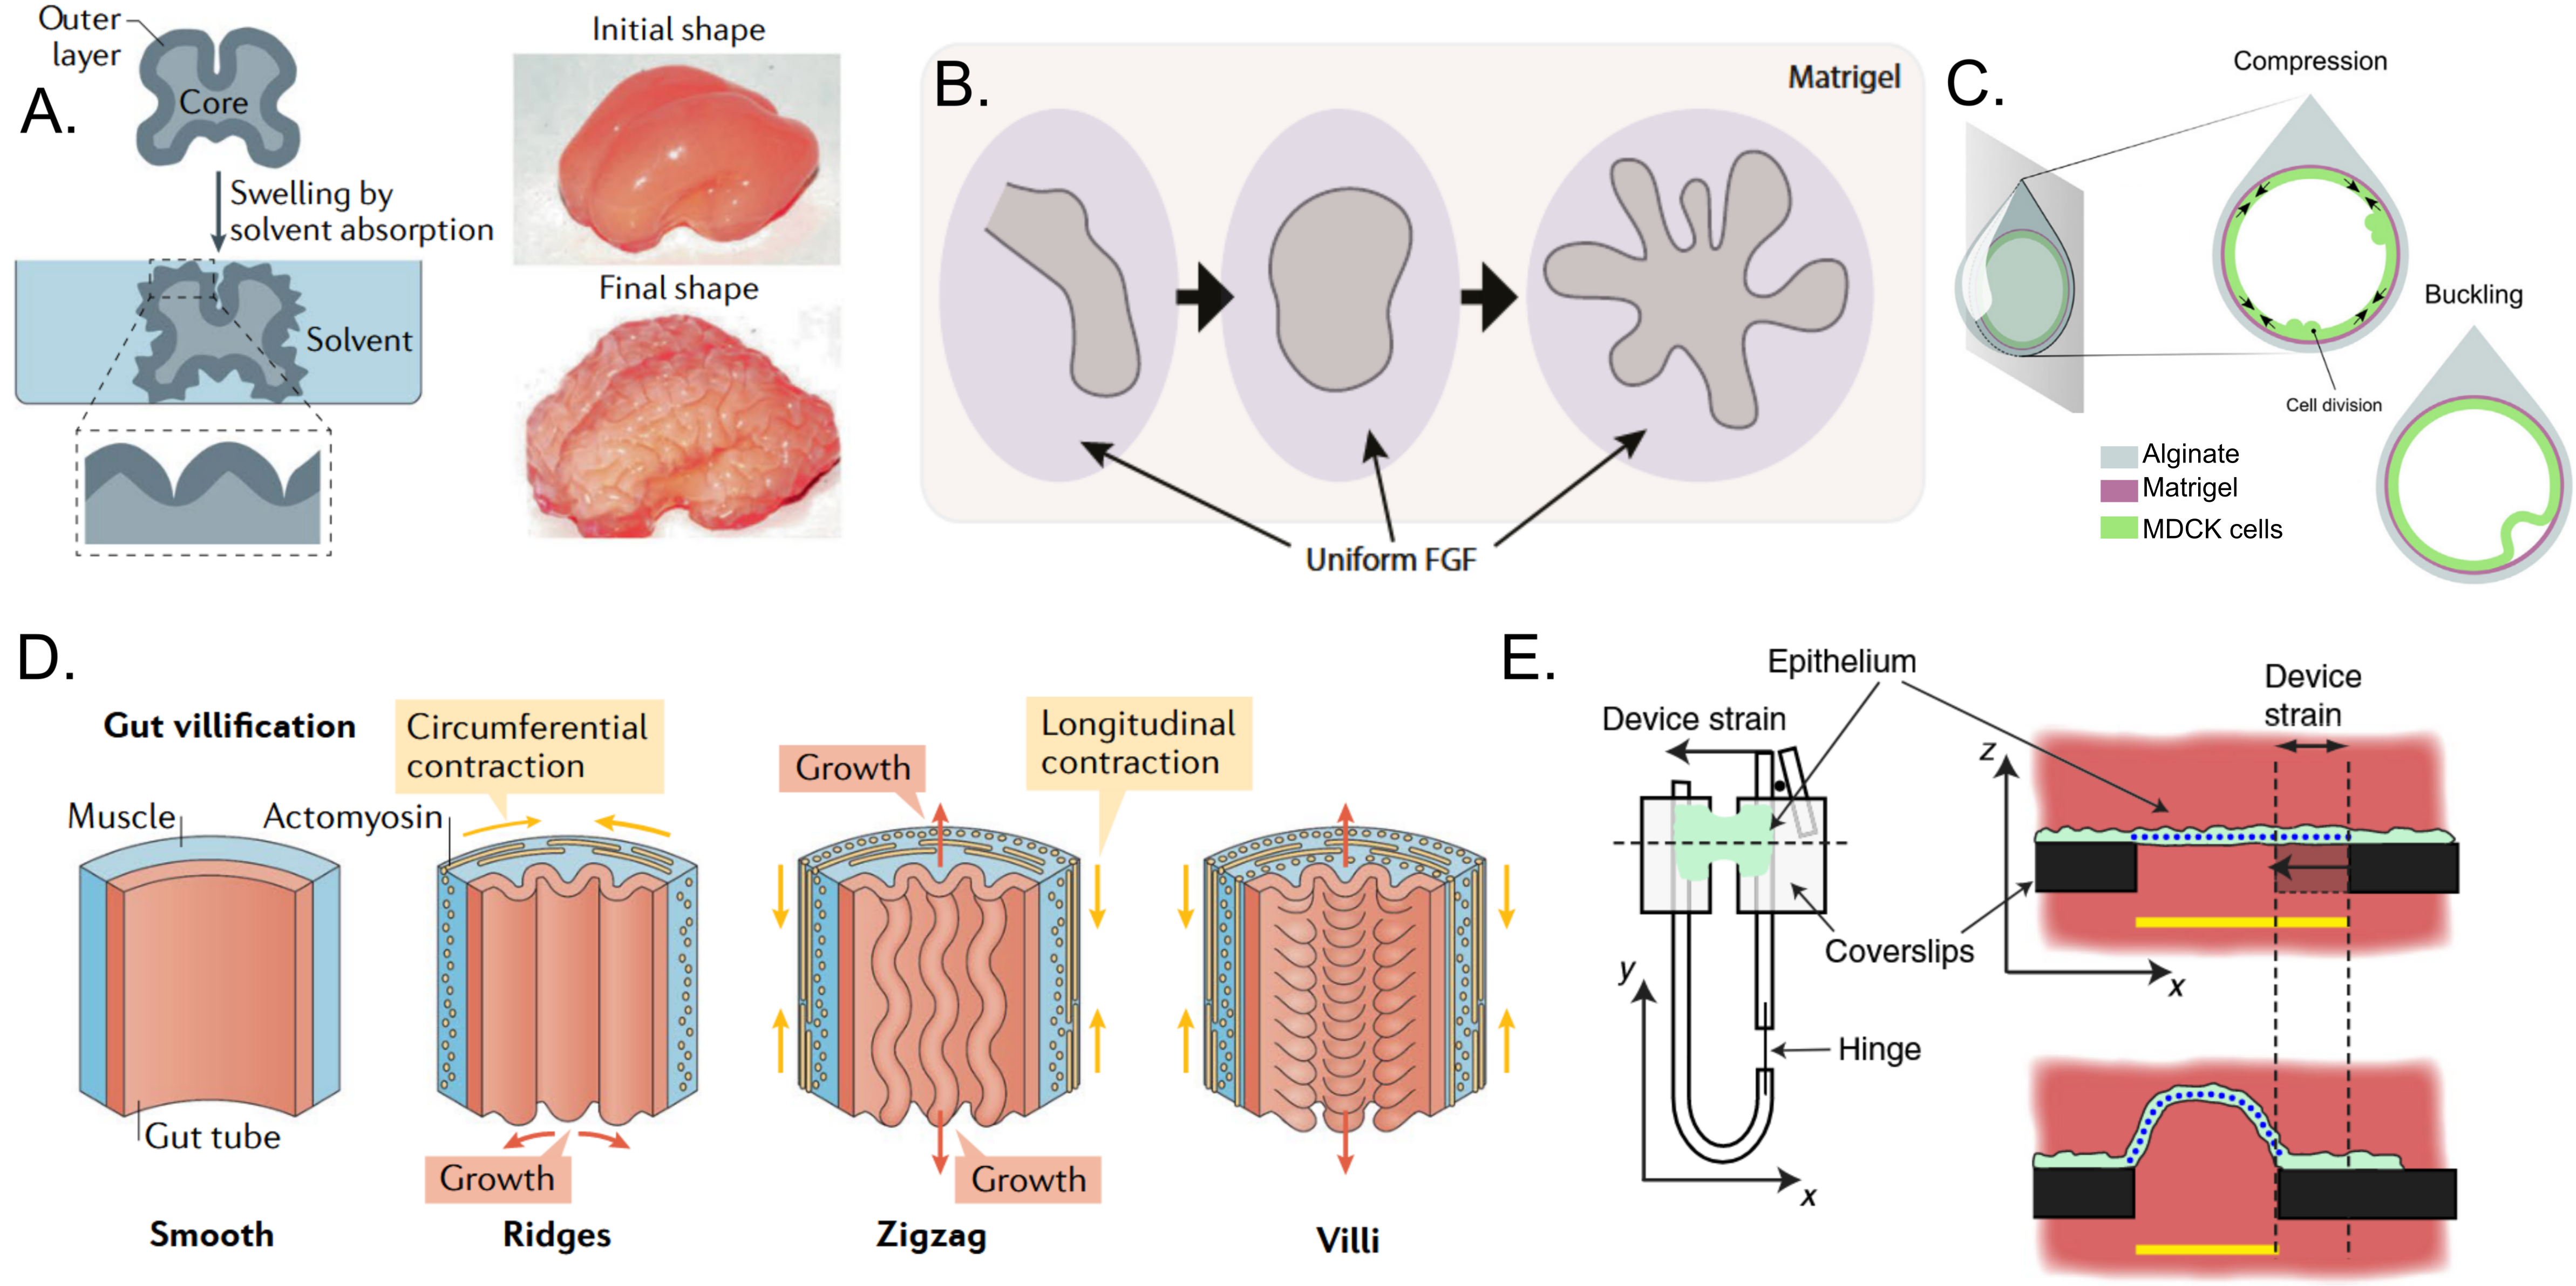
\includegraphics[width=\textwidth]{chap4buckling.png}
	\caption{\label{fig_4_6} \textbf{Examples of mechanical instabilities}: (A) Synthetic mini brains illustrate the wrinkling of the outer layer with swelling mimicking gyrification \cite{tallinen2016}. (B, D) Other way around where inner layer of lung or intestinal epithelia develops folds when embedded into a hydrogel or muscle shell \cite{varner2015, shyer2013}. (C) It is also shown that simple epithelial tissues embedded into a shell would also buckle \cite{trushko2020}. (D) \cite{wyatt2020} used matrix independent tissue with compression to illustrate that the epithelial tissue itself can undergo buckling. \textit{Panel A, D are adpated from \cite{collinet2021} and C from \cite{matejcic2020}}
	}
\end{figure}

The formation of the ventral furrow in the drosophila embryo can also be considered as a buckling event. Although there are multiple explanations for this phenomenon, recent studies have shown that the instability leading to the fold is caused by embryo-level forces \cite{guo2022, fierling2022}. Apart from instabilities, it is remarkable that the mechanical information can be encoded in the substrate. For instance, the tension produced by the cells in a pre-stretched membrane, on cutting would lead to curling \cite{tomba2022}, or through stretching a suspended epithelial layer would also do the same\cite{fouchard2020}.

It is noteworthy that there is currently only one established method for directly applying compressive stresses to suspended epithelial tissue. The Lab of Guillaume Charras has developed a technique using a cell-laden collagen gel sandwiched between two rods, where the gel is digested with collagenase to create a suspended monolayer (see fig \ref{fig_4_6} E). Through extensive experimentation, they have observed that the compression of more than 35\% strain produces transient buckling events \cite{wyatt2020}. Importantly, the actin cytoskeleton plays a crucial role in buffering deformations in this system.

\hypertarget{tissue-hydraulics}{%
	\section{Tissue hydraulics}\label{tissue-hydraulics}}

\hypertarget{hydraulic-control-of-morphogenesis}{%
	\subsection{Hydraulic control of morphogenesis}\label{hydraulic-control-of-morphogenesis}}


\begin{figure}
	\centering
	\includegraphics[width=\textwidth]{chap4hydraulics.png}
	\caption{\label{fig_4_7} \textbf{ Tissue hydraulics} plays an essential role in establishing (A) embryonic axis through lumen coarsening, and later the pressure regulates the size of the embryo. Laplace's law acts on the spherical cavities between cells to the whole blastocyst \cite{dumortier2019,chan2019, collinet2021}. (B) Interestingly, if the inflated structure is surrounded by a mesh you see a stressball effect, where material inflates through the mesh. Similar phenomena is visible in growth and inflation of the lizard lungs. The smooth muscle constrains the deformation leading to stressball morphogenesis \cite{palmer2021}. (C) In cnidarians, the different orientation of F-actin leads to different shapes of the organism \cite{stokkermans2022}.
	}
\end{figure}

In this thesis, we focus on the role of hydraulic pressure in morphogenesis. It has been well established in the field of developmental biology that fluid pressure plays a significant role in lumen expansion. For instance, in the mouse embryo, cell aggregates form small fluid cavities in intercellular junctions, which grow and coalesce into a large lumen, breaking the symmetry of the embryo, due to the presence of an osmotic pressure gradient (\cite{dumortier2019}; reviewed by \cite{torres-sanchez2021}, see fig \ref{fig_4_7} A). This process is powered by the pumping of ions and water by the cells, which generates pressure in the fluid-filled cavities, ultimately leading to the formation of spherical embryos. For any inflated spherical shell, the relationship between pressure ($\Delta P$), curvature ($R$), and surface tension ($\sigma$) can be described by Laplace's law. 
$$ \sigma = \frac{\Delta P R}{2}. $$ 
The shape that is created under pressure depends on the material properties of the tissue. For example, a homogeneous material would create a uniform curvature, such as a spherical shape, while an anisotropic tissue with oriented cells would result in various shapes, such as cylinders or ellipsoids \cite{stokkermans2021} (see fig\ref{fig_4_7} C). An interesting example of this phenomenon can be seen in the lobed epithelium of lizard lungs, which resembles the shape of a stress ball. Palmer et al. propose that the smooth muscle network functions as a mesh that constrains the epithelium, much like the outer layer of a stress ball \cite{palmer2021} (see fig\ref{fig_4_7} B). Upon the application of pressure, the epithelium inflates in the regions between the gaps in the muscles.

For embryos, an increase in pressure results in an increase in tension and stretching of the cells. Once a certain threshold is reached, the cell junctions may leak, causing a reduction in luminal pressure and shrinkage of the embryonic cavity. This system of pressure regulation through leakage acts as a mechanism for size regulation \cite{chan2019}. At the same time, it polarizes the embryo and promotes cell segregation and fate specification (see fig\ref{fig_4_7} A, reviewed by \cite{chan2020}).

Similar coalescence and lumen coarsening have been observed in other systems (reviewed in \cite{schliffka2019}). The pressure can also be generated through secretion of the matrix, as seen in the case of the drosophila hindgut with mucins \cite{syed2012}, or through the secretion of hyaluronic acid in the formation of ear canals in zebrafish otic vesicles \cite{munjal2021}. Despite numerous
\textit{in vivo} experiments, there are very few systems in which epithelial tissue can be subjected to controlled shape and size \textit{in vitro}.

\hypertarget{mechanics-of-domes}{%
	\subsection{Mechanics of domes}\label{mechanics-of-domes}}

\begin{figure}
	\centering
	\includegraphics[width=\textwidth]{chap4domes.png}
	\caption{\label{fig_4_8} \textbf{Historical development of epithelial domes}:(A) Distended epithelium was observed in explant cultures in 1930-50s. (B) With MDCK cell line, spontaneously forming domes/hemicysts were characterized \cite{leighton1969, valentich1979}. (C,D) In our lab, shape and size of the domes were controlled with micropatterning adhesion protein \cite{latorre2018}. The pressure and tension was measured with Laplace's law and traction force microscopy. (E-F) For non-spherical domes, curved monolayer stress microscopy technique was implemented by segmenting the dome shape \cite{marin-llaurado2022}.
	}
\end{figure}

Many of the morphogenetic events are called doming because the shape vaguely resemble a spherical cap. For instance, doming of the retina in the eye or zebrafish embryo, or doming during duct formation of mammary or salivary glands. There are typically two mechanisms for these: first, an accumulation of the cells or matrix to create curvature; and second, trans-epithelial transport causing hydraulic pressure-driven shape change. The second kind is remarkable as they mimic various lumenized epithelia \textit{in vivo}.

This is the most pertinent system to the thesis. I would briefly go into the historical developments in dome mechanics. 
	
Fluid-filled dome formation in epithelial tissue culture has been recorded since 1933 \cite{cameron1953} (see fig \ref{fig_4_8} A). After several decades alongside the development of cell culture techniques, microscopy, and MDCK cell line \footnote{It is very important to acknowledge the contribution of Madin-Darby canine kidney (MDCK) cells to the field of mechanobiology and enhancing our understanding of tissues \textit{in vitro}. Stewart H. Madin and Norman B. Darby, Jr. isolated female cocker spaniel dog’s kidney tubules cells in 1958. MDCK cells can self-organize in 2D and 3D; form monolayers and stratified layers; and undergo collective migrations. These cells are incredibly robust for experimentation.}, in 1968, Leighton and colleagues observed that the confluent MDCK cell monolayers formed hemispherical blisters (domes) \cite{leighton1969} (see fig \ref{fig_4_8} B). They observed that these are different from renal tubules because the apical surface, with microvilli, was facing outwards. They saw that these fluid-filled structures are dynamically changing size and curvature. They would burst to deflate and leak fluid out in the medium \cite{valentich1979}. After sometime, they could heal and form the dome again. Later, other cell lines derived from mammalian and amphibian kidneys were often observed to form domes too \cite{dulbecco1980, leighton1981, lever1979}
	
Now the mechanism is clear as the epithelial cells perform critical barrier function alongside controlling the transepithelial flow of ions and water. It was shown that hindering sodium-potassium ion pumping reduces the likelihood of domes \cite{leighton1969}. Thus, on forming a confluent monolayer these cells perform their function of pumping ions from apical to basal direction \cite{valentich1979}. If the substrate is solid and impermeable the tissue accumulates enough pressure to delaminate and form a spherical structure.

Most domes observed have been spherical and circular in footprint, indicating uniform tension across the dome. This can be explained by considering the dome as a thin shell under pressure, similar to a bubble, and following Laplace's law. Early studies attempted to infer tension through geometry and pressure measurement \cite{tanner1983}, finding that the pressure was of the same order as physiological vessels (see fig \ref{fig_4_9} A-B).

\begin{figure}
	\centering
	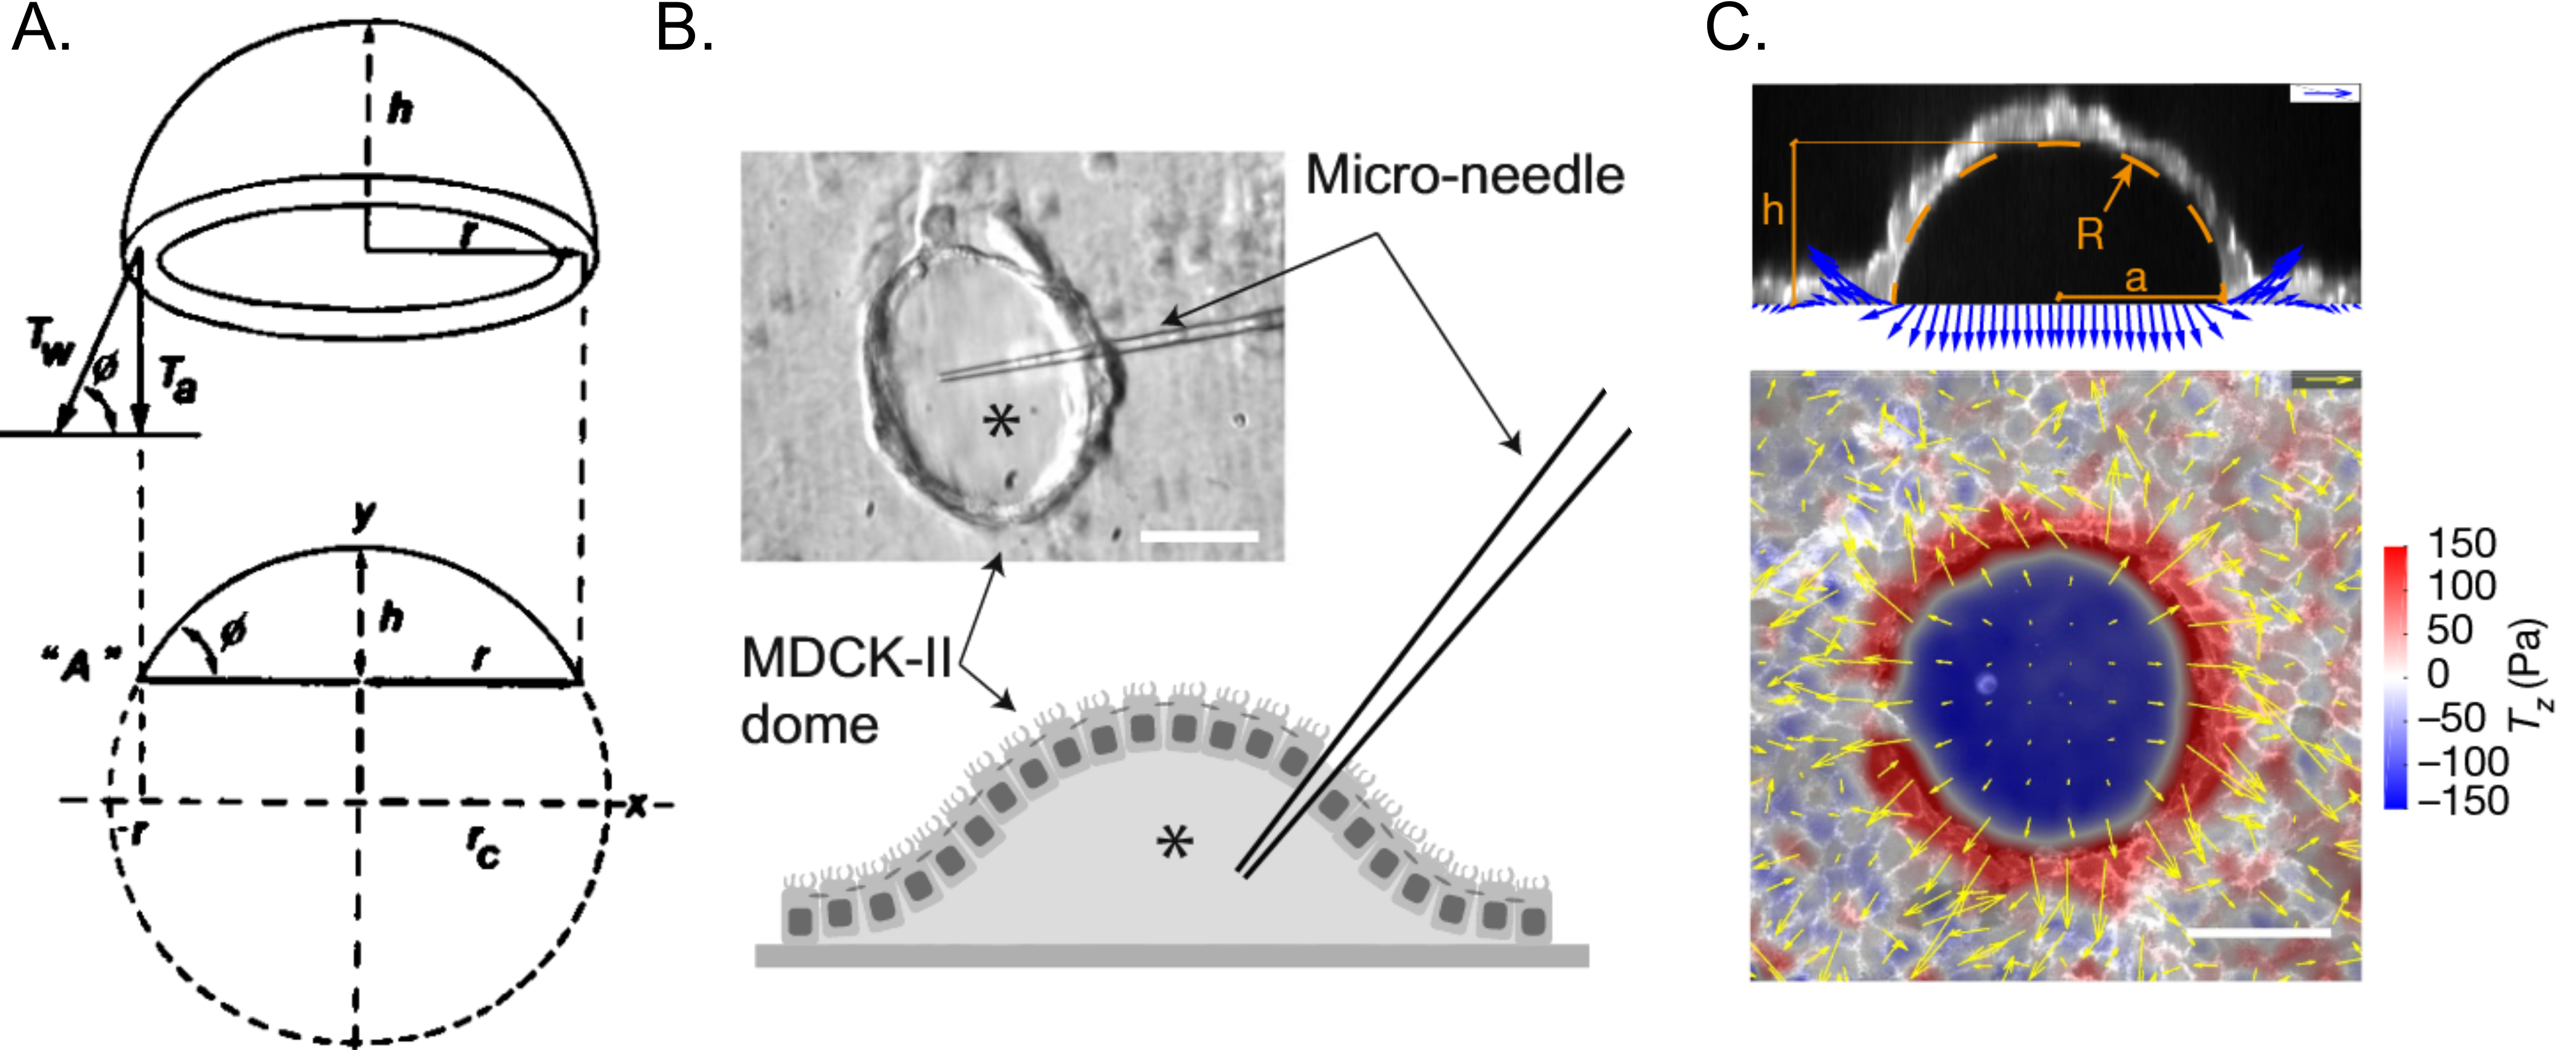
\includegraphics[width=\textwidth]{chap4pressure.png}
	\caption{\label{fig_4_9} \textbf{Methods for measuring pressure and tension}: (A) Earlier studies tried to estimate tension through geometry and thickness of the monolayer \cite{tanner1983}. (B) Later, pressure was measured by puncturing the dome with a micro-needle. However, the measurement of pressure is static, because the dome deflated after the puncturing \cite{choudhury2022}. (C) Traction force microscopy technique provides a viable non-invasive solution for measuring pressure under to domes \cite{latorre2018}.
	}
\end{figure}

One study \cite{popowicz1986} identified a ``dome curve'' when the frequency of domes was plotted against size, observing three classes of domes in terms of size. Smaller domes were observed to swell and increase in size. It was also suggested that there could be different subpopulations of MDCK cells. In the 1990s, many strains were characterized that formed different inflated structures, ranging from normal domes to tubules \cite{klebe1995}. One cell line, called super dome MDCK, formed larger domes.

Despite research into ion transport, hormone signaling, the role of tight junctions, and external shear stress, the understanding of the mechanics of domes and pressure has remained stagnant due to the lack of tools for measuring tension, pressure, and controlling the shape and size of these structures.

The work of Ernest Latorre in our laboratory has led to the development of a system for controlling the size of domes and studying the relationship between tension and pressure \cite{latorre2018} (see fig \ref{fig_4_8} C-D). By utilizing protein patterning techniques, Latorre was able to create non-adhesive circular regions on soft PDMS gel, which, when seeded with MDCK cells, led to the formation of domes. The gel was embedded with beads to allow for the calculation of traction forces and pressures exerted by the monolayer (see  fig \ref{fig_4_9} C). This system allowed for a deeper understanding of the rheology of tissue and the role of the cytoskeleton. He observed that stretching the actin cortex leads to dilution, and that tension reaches a stable value regardless of strain. He also observed the surprising phenomenon of superelasticity, where cells are heterogeneously stretched in the dome when tension is uniform. To further understand the role of actin and keratin bundles in providing superelasticity, Latorre et al. developed a vertex model through which they could understand the instability triggered by actin dilution, and rescued by intermediate filaments.

Ariadna Marin-Llaurado extended Latorre's work by examining domes of varying sizes and shapes (see fig \ref{fig_4_8} E). This study found that different-sized spherical domes have similar tensions, and that pressure is compensated according to curvature. Marin-Llaurado couldn't rely on a simple formula for tension calculation, because the tension in non-spherical domes is non-uniform \cite{marin-llaurado2022}. They used confocal microscopy to map dome curvature and calculated stresses computationally using a novel method called cMSM (curved Monolayer Stress Microscopy) (see fig \ref{fig_4_8} F). This method infers stresses just through geometry and pressure as in Young-Laplace relation. It does not need to make any assumptions related to material properties. The results showed that cells tended to align along the principal stress direction.

The mechanics of osmotic and hydraulic gradients are also crucial to understand. Chaudhary et al.~demonstrated that kidney cells act like a mechanobiological pump \cite{choudhury2022}. Using a two-layer microfluidic chip, the team was able to measure and apply pressure differences across an epithelial monolayer and observe that the tissue acted like a mechanical pump that stalls at high pressure. Remarkably, they discovered that diseased kidney cells pump in a different direction than healthy ones. They were able to control both osmotic and hydraulic pressure. Another study by Ishida-Ishihara et al.~investigated the connection between osmotic pressure and extracellular matrix swelling \cite{ishida-ishihara2020}. The researchers found that osmotic gradients trigger Aquaporin transport channels, leading to dome formation through Matrigel swelling. However, these domes are gel-filled structures that  differ from fluid-filled domes.

MDCK domes provide a model system for studying transport, cell fate, and tissue dynamics with a curvature. However, control over luminal pressure in these structures remains a challenge.

\hypertarget{what-is-to-be-done}{%
	\section{What is to be done?}\label{what-is-to-be-done}}

Morphogenesis refers to the process of tissue deformation or growth, which results from the combination of both endogenous and exogenous mechanical forces \cite{valet2022, collinet2021}. These forces may arise from the contractility of the epithelium and the surrounding matrix, as well as hydraulic pressure from the lumen \cite{torres-sanchez2021, chan2020}. The various stresses act on different components of the tissue, such as cells and the extracellular matrix, which exhibit unique viscoelastic properties and remodeling time scales \cite{cavanaugh2020, kelkar2020, ambrosi2019}. However, comprehending how these stresses interact with viscoelastic properties to bring about particular morphogenetic events in vivo presents significant technical and conceptual challenges. These obstacles include disentangling the roles played by distinct components in a system, a lack of tools for quantitative measurements of stresses and mechanical properties, and an inability to apply controlled stresses over a wide range of amplitudes and rates.

In response to these challenges, bottom-up approaches have emerged as a complementary strategy for understanding the morphogenetic potential of individual components and building complex, functional tissues \cite{trentesaux2023, ingber2018}. These approaches have been successful in engineering basic morphogenetic processes such as epithelial bending or buckling \cite{matejcic2022}. However, even though bottom-up approaches are proving to be successful, we still need tools that can measure and control the shape and stress of 3D epithelia simultaneously. Additionally, we lack computational models that integrate cellular and tissue shape with the subcellular determinants of epithelial mechanics, such as the contractility, turnover, and viscoelasticity of the actomyosin cortex.

This thesis seeks to address these gaps in knowledge by investigating the mechanics of epithelial tissues. A comprehensive understanding of the principles that govern tissue form and function is essential for both advancing our understanding of fundamental physical rules in biology and inspiring new engineering tools and design principles. To achieve this, we leverage cutting-edge technologies, such as 3D printing, microfluidics, and 3D cell cultures, to individually control morphogenetic driving factors. 

Our approach provides a material science perspective for probing the intricate mechanisms involved in the generation of forces and shape changes at the cellular and tissue levels, and holds promise for discovering emergent phenomena and enabling the building of novel tissue forms and assemblies.  
